%% ----------------------------------------------------------------
%% Introduction.tex
%% ---------------------------------------------------------------- 
\chapter{Introduction} \label{Chapter:Introduction}
%The Introduction to my Report \dots

%The initial idea of the project was taken from Pirobot(\cite{Pirobot}).
%
%\inote{what it will do. Define everything. Use. Very general}
%General - mapping robots. 
%
%stereovision - uses etc.
%
%other similar projects
%
%why mine is important 

\inote{Talk about what I set out to do, include some definitions etc. }
\inote{What I ended up doing}
\inote{The uses of my robot.} 

\begin{figure}
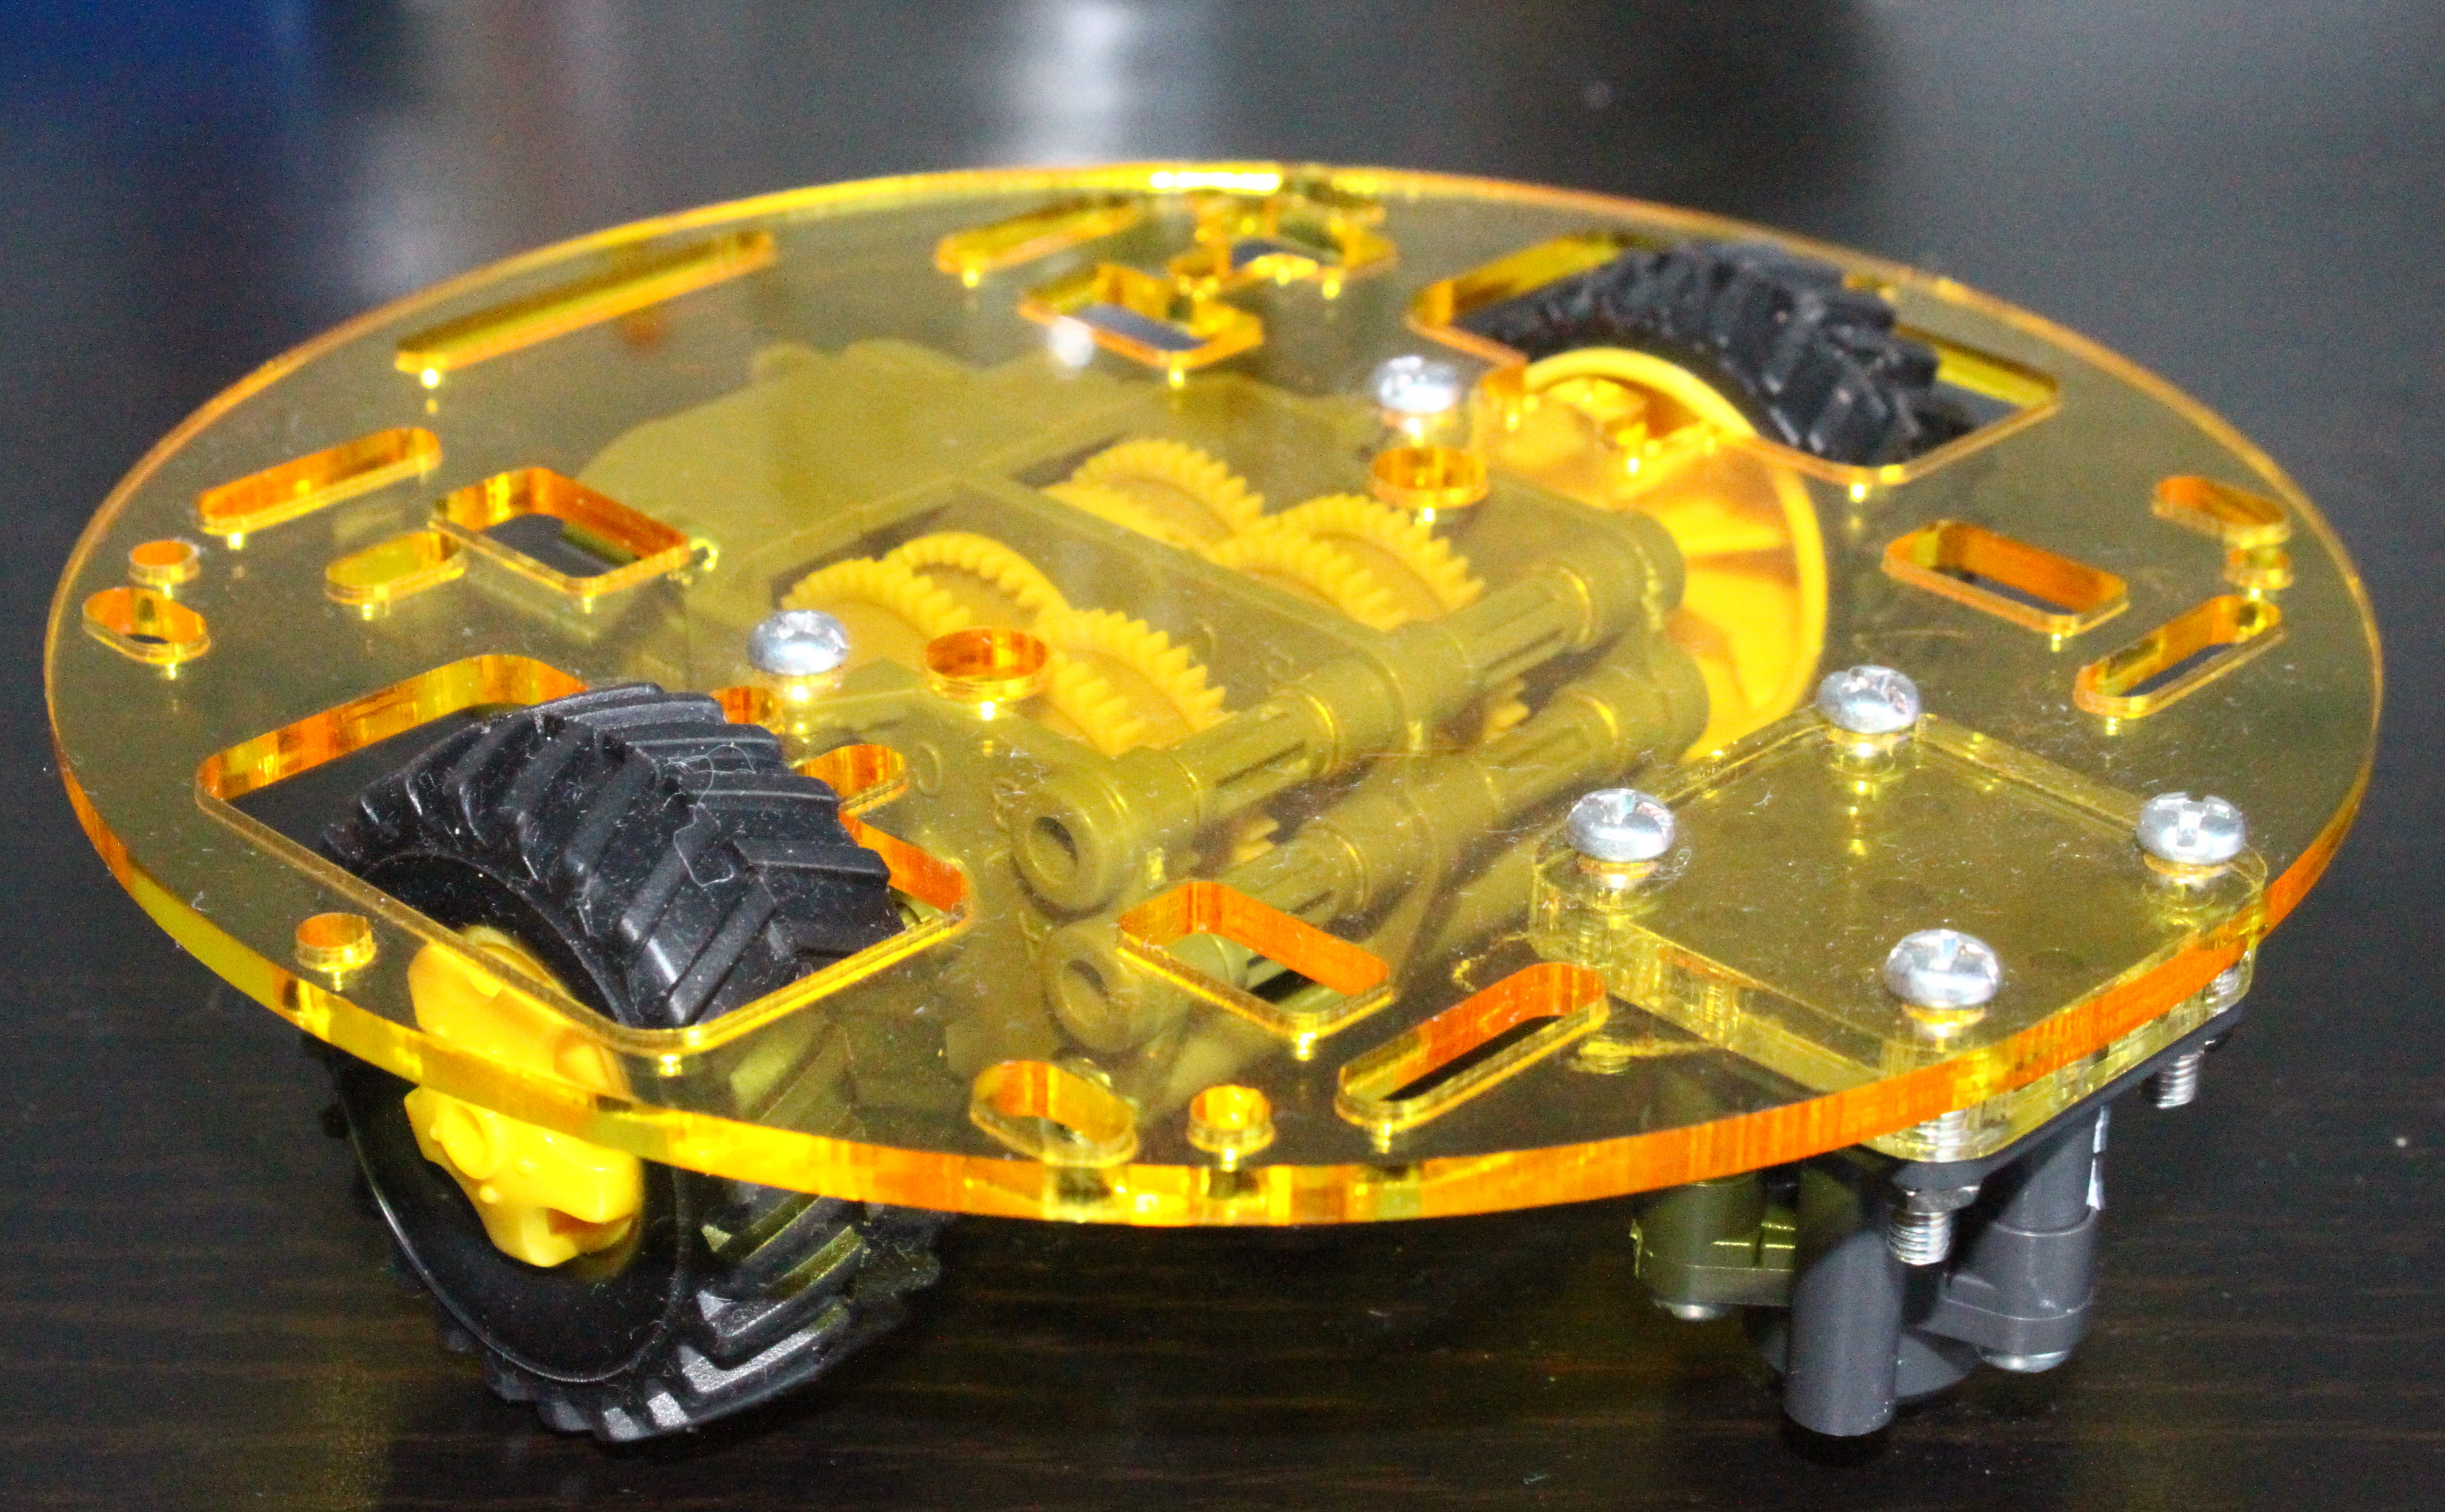
\includegraphics[width=\textwidth]{./Figures/RobotBase.jpg}
\caption{The base of the robot}
\label{fig:RobotBase}
\end{figure}

\section{Project Management}
In order to reduce the risk within the project, all aspects of potential issues are looked at and are summarised in table \ref{tab:risk}. A Gantt chart of how time will be spent can be seen in figure \ref{fig:Gantt}. 

The project will be designed in stages - first, gaining operation of all the basic sections; movement, image capturing, image detection algorithms etc. These will then be brought together once tested to create the final product. 
\begin{table}
\begin{tabular}{|p{6cm}|p{2cm}|p{6cm}|}\hline
Risk						&	Severity	&	Prevention \\ \hline
Parts not arriving on time	&	High		&	Order parts as early as possible \\
Project not fulfilling specification				&	High		&	Develop in stages to obtain functionality in parts. Ensure enough time is allocated to the project.	\\
PCB Design is incorrect		&	Medium		&	Check the design carefully and get second opinion \\
Failure of personal computer causing data loss & Low	& 	Keep back ups of all work on Devtrack Git repository and Dropbox.\\

\hline
\end{tabular}
\caption{A list of risks and the prevention steps taken to reduce their impact}
\label{tab:risk}
\end{table}
